%
% Introdução
%
\section*{Introdução} \label{Introducao}

Com a explosão da \textit{Internet of Things (IoT)} nos dias de hoje, as pessoas ainda realizam tarefas no seu dia-a-dia que poderiam ser auxiliadas por recursos mais inteligentes. Libertando-o para outras atividades como lazer. Ao automatizarmos a recolha de dados relacionada com os stocks de produtos em casa, conseguimos dinamizar a eficiência na gestão dos mesmos, ajudando os utilizadores a manter o stock adequado às suas necessidades, bem como alerta-lo para a falta de produtos. Assim, o nosso trabalho vai no sentido de dar repostas a ``como evitar transtornos causados na altura de reabastecer a nossa despensa? controlo de stock de alimentos e outros produtos? artigos fora de prazo?". Se entendermos que a nossa casa funciona como uma empresa, onde existem pessoas que podem realizar as mesmas tarefas, e.g. ir às compras seguindo uma lista previamente elaborada, capacitamos qualquer elemento da família para exercer a compra.

Para responder às perguntas levantadas anteriormente, pretendemos desenhar duas aplica-ções, uma móvel e uma web, que interagem diretamente com uma Web API. A recolha de dados, i.e., informação dos produtos existentes, é feita por um leitor de {\itshape tags} (NFC ou RFID) e transmitida para a Web API, para ser armazenada. Os locais de armazenamento de produtos devem dispor de dispositivos de hardware, equipados com scanners capazes de ler as {\itshape tags} e sensores de movimento. A adoção destas peças é a chave na monitorização dos stocks, permitindo a distinção do tipo de movimento, de entrada ou saída.

No âmbito do nosso projeto assumimos a existência de dois estados para os produtos, avulsos e embalados. Os primeiros são conservados em sistemas de arrumação (caixas, sacos, etc.), que contém {\itshape tags} NFC programáveis por {\itshape smartphones}. Os detalhes dos produtos são especificados pelo utilizador e carregados para a {\itshape tag}. Enquanto que para os produtos embalados, admitimos que os produtores utilizam {\itshape tags}, NFC ou RFID, para guardar os rótulos em formato standard.


\vspace{-15mm}
\hspace{2mm}

\begin{figure}[h!]
	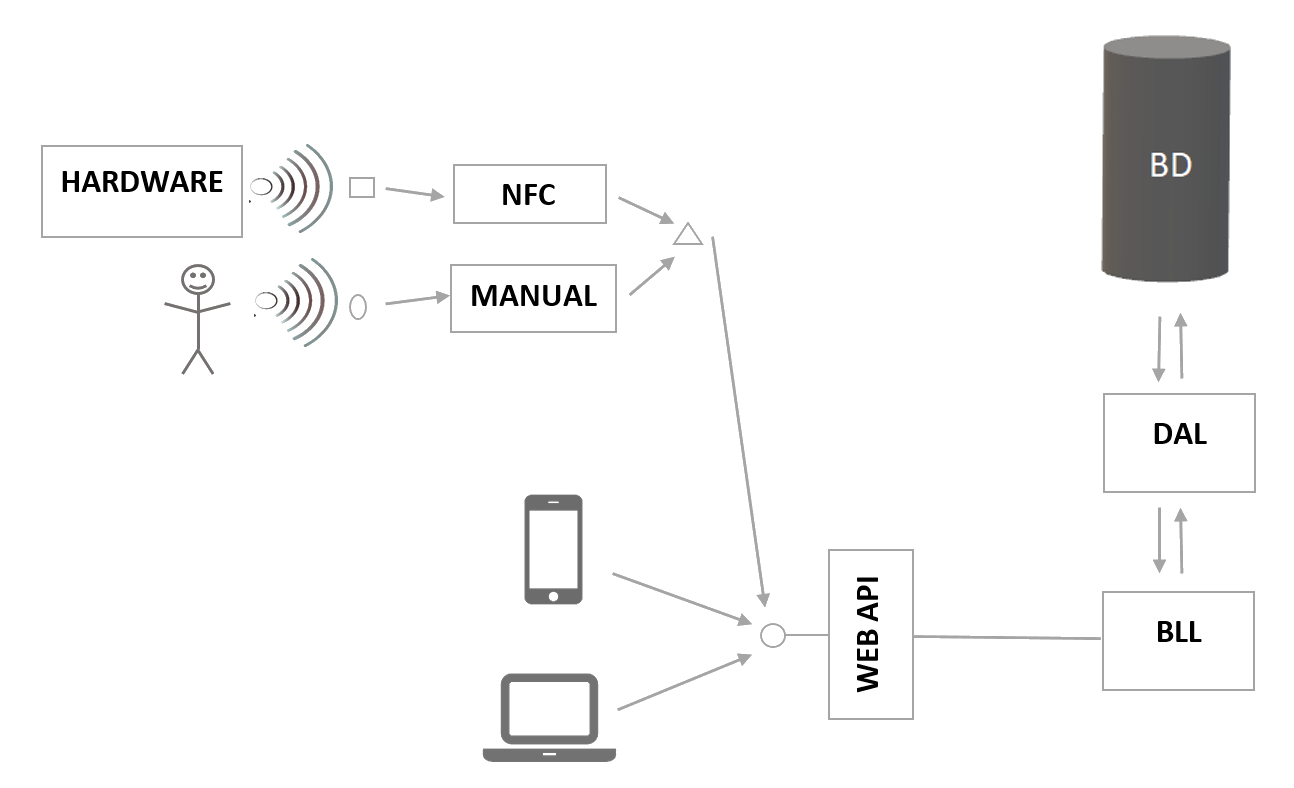
\includegraphics[width=14cm,height=7.5cm,scale=0.5]{./figures/Esquema_Estrutura_Projeto_Geral.png}
	\caption{Esquema Geral do Projeto}
	\label{esquema_geral}
\end{figure}

